\documentclass[UTF8, a4paper, 12pt]{ctexart}

\usepackage{amsmath,amssymb}
\usepackage{geometry}
\usepackage{booktabs}
\usepackage{hyperref}
\usepackage{graphicx}
\usepackage{float}
\usepackage{array}
\usepackage{tabularx}
\usepackage{enumitem}

\geometry{left=2.5cm, right=2.5cm, top=3.0cm, bottom=3.0cm}
\hypersetup{colorlinks=true, linkcolor=blue, citecolor=green}

\newcommand{\Log}{\mathrm{Log}}

\title{\textbf{无人机机械臂末端位姿稳定\\项目说明（简化版）}}
\author{周子涵}
\date{\today}

\begin{document}
\maketitle

\begin{abstract}
本文档为《项目设计说明》的简化版，概述空中机械臂末端稳定系统的目标、架构、三控制模式及主要实验结论。完整技术细节、公式推导与参数表见 \texttt{docs/main.tex}（PDF：\texttt{docs/pdf/项目说明.pdf}）。
\end{abstract}

\clearpage
\tableofcontents
\clearpage

%==============================================================================
\section{项目概述}
%==============================================================================

\subsection{背景与目标}

在无人机--机械臂系统的实际作业中，无人机基座常因气流扰动、突发风载或机身晃动产生动态耦合扰动。机械臂末端需在世界系中保持恒定，以完成抓取、维护或观测等任务。本项目通过关节主动补偿基座运动，实现末端位姿稳定。

启动时锁定世界系目标 $T_E^*$，通过
\begin{equation}
    T_D = T_B^{-1}\, T_E^*, \qquad T_E \approx T_E^*,
\end{equation}
将``世界系保持''转化为基座系中对时变期望 $T_D$ 的跟踪。$T_B$ 为基座位姿，$T_D$ 为基座系期望末端位姿。

\subsection{设计要点}

\begin{itemize}[leftmargin=2em]
    \item 世界系锁定 $T_E^*$，不随基座漂移；
    \item 规划、控制、执行三层解耦；
    \item 三种模式共享同一规划层（$T_D,V_D$），便于对比与故障分层；
    \item $V_D$ 采用解析速度生成，避免仿真/真机频率差异下数值差分的相位延迟。
\end{itemize}

%==============================================================================
\section{系统架构}
%==============================================================================

\begin{figure}[H]
    \centering
    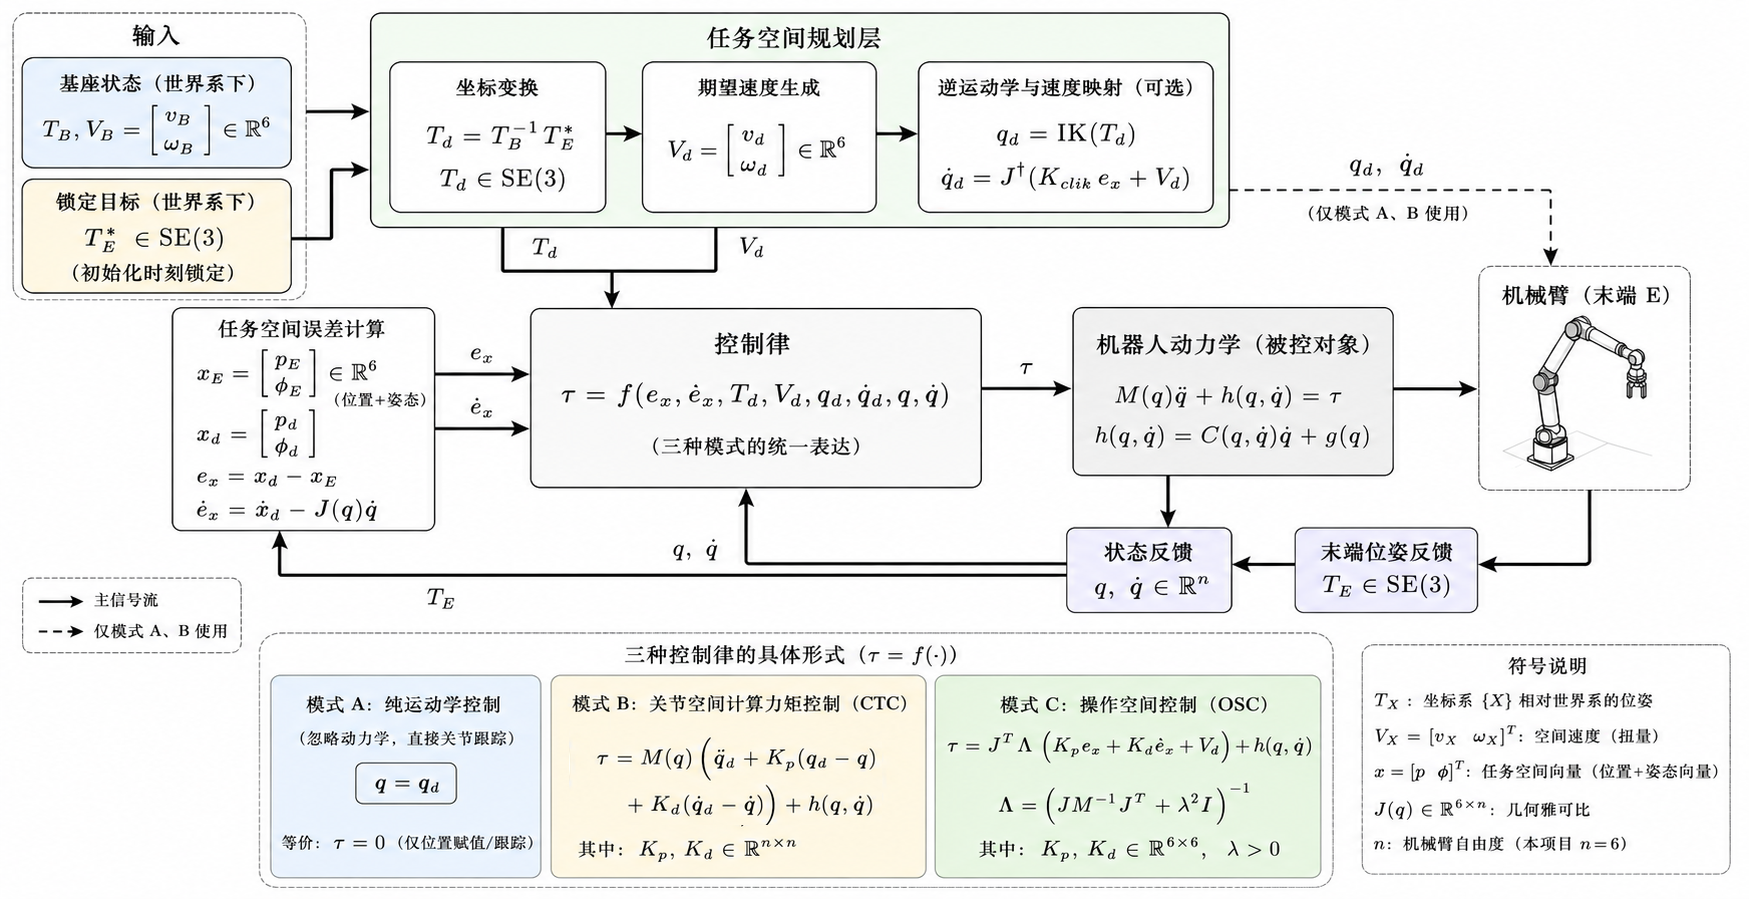
\includegraphics[width=0.95\linewidth]{1.png}
    \caption{三层架构：规划 $\rightarrow$ 控制 $\rightarrow$ 执行}
\end{figure}

\begin{table}[H]
  \centering
  \caption{三种控制模式}
  \renewcommand{\arraystretch}{1.2}
  \begin{tabular}{@{} l l l l @{}}
    \toprule
    模式 & 名称 & 控制目标 & 真机角色 \\
    \midrule
    A & Kinematic Control & 几何极限（$q=q_D$） & 规划层 Benchmark \\
    B & CTC & $q \rightarrow q_D$ & 关节动力学评估 \\
    C & OSC & $T_E \rightarrow T_D$ & \textbf{部署主方案} \\
    \bottomrule
  \end{tabular}
\end{table}

规划层输出 $T_D,V_D,q_D,\dot{q}_D$；三种模式共用该输出，仅在控制层与执行层不同。单周期数据流（以模式 C 为例）：读取 $q,\dot{q}$ 与 $T_B$ $\rightarrow$ 计算 $T_D,V_D,e_x$ $\rightarrow$ OSC 输出 $\tau$ $\rightarrow$ 执行层更新 $q,T_E$。

%==============================================================================
\section{规划层}
%==============================================================================

规划层在基座运动时，根据世界系锁定目标计算关节参考 $q_D,\dot{q}_D$ 及任务空间量 $T_D,V_D$。该层与控制律无关，三种模式共用同一套计算。

\subsection{输入与输出}

\begin{table}[H]
  \centering
  \caption{规划层接口}
  \renewcommand{\arraystretch}{1.2}
  \begin{tabularx}{\textwidth}{@{} l X @{}}
    \toprule
    输入 & 说明 \\
    \midrule
    $T_B$、mount 速度 & 仿真由内置 mount 模型给出；真机由飞控 TF 提供 \\
    $T_E^*$ & 启动时锁定的世界系目标位姿 \\
    $q,\dot{q}$ & 当前关节状态（用于 IK/CLIK） \\
    \midrule
    输出 & 说明 \\
    $T_D,V_D$ & 基座系期望末端位姿与补偿速度 \\
    $q_D,\dot{q}_D$ & 关节参考（模式 A/B 跟踪；模式 C 仅遥测） \\
    \bottomrule
  \end{tabularx}
\end{table}

\subsection{世界系锁定与基座系目标}

系统启动时记录末端位姿 $T_E(t_0)$，令 $T_E^*$ 此后不变。每个控制周期根据实时基座 $T_B$，将世界系目标换算到基座系：
\begin{equation}
    T_D = T_B^{-1}\, T_E^*.
\end{equation}
无人机带着机械臂移动时，若要在地面上``钉住''末端，机械臂必须在基座系中做反向运动；$T_D$ 即该反向运动的位姿目标。

\subsection{任务误差与期望速度}

在基座系中比较期望与实际末端，定义六维任务误差：
\begin{equation}
    e_p = p_D - p_E, \quad
    e_R = \Log(R_E^\top R_D), \quad
    e_x = [e_p;\, e_R].
\end{equation}
同时计算期望 twist $V_D$（线速度 + 角速度），用于补偿基座运动。本系统采用\textbf{解析速度}：由当前 mount 运动直接算出 $V_D$，不对 $T_D$ 做数值差分，以避免仿真（500\,Hz）与真机（100\,Hz）频率不一致带来的滞后。

\subsection{逆运动学与关节速度前馈}

规划层还需将任务空间目标转为关节参考，供模式 A/B 使用（模式 C 的 OSC 不跟踪 $q_D$，但仍并行计算作遥测）。

\textbf{逆运动学（IK）}：用阻尼最小二乘（DLS）在速度层求关节角速度
\begin{equation}
    \dot{q} = J^\top (JJ^\top + \lambda_{\mathrm{IK}}^2 I)^{-1} e_x,
\end{equation}
再离散积分 $q\leftarrow q+\alpha\dot{q}$ 迭代至收敛，得到 $q_D$。

\textbf{CLIK 速度前馈}：运行时给出关节期望速度
\begin{equation}
    \dot{q}_D = J^\top (JJ^\top + \lambda_{\mathrm{CLIK}}^2 I)^{-1}(K_x e_x + V_D),
\end{equation}
其中 $K_x e_x$ 为误差反馈，$V_D$ 为基座补偿前馈。

%==============================================================================
\section{控制层}
%==============================================================================

控制层将规划层给出的 $T_D,V_D$ 转化为关节运动或力矩指令。三种模式共用规划层输出，差异在于闭环空间与优化目标。

\subsection{三种模式概览}

\begin{table}[H]
  \centering
  \caption{控制层分工}
  \renewcommand{\arraystretch}{1.2}
  \begin{tabular}{@{} l l l @{}}
    \toprule
    模式 & 控制思想 & 信号链 \\
    \midrule
    A & 几何极限 & $T_D,V_D \rightarrow \mathrm{IK} \rightarrow q_D \rightarrow q$ \\
    B & 关节空间跟踪 & $T_D,V_D \rightarrow \mathrm{IK} \rightarrow q_D \rightarrow \mathrm{CTC} \rightarrow \tau$ \\
    C & 任务空间调节 & $T_D,V_D \rightarrow e_x \rightarrow \mathrm{OSC} \rightarrow \tau$ \\
    \bottomrule
  \end{tabular}
\end{table}

\subsection{模式 A：Kinematic Control}

假设关节能瞬间到达 IK 输出，直接令 $q=q_D$、$\tau=0$，不积分动力学。该模式给出规划链路的\textbf{几何性能上界}（本项目位置 RMS 0.283\,mm）：任何考虑惯性、力矩限幅的方案不应系统性优于 A。用于标定规划层与 Benchmark。

\subsection{模式 B：CTC（计算力矩控制）}

在\textbf{关节空间}闭环，目标是 $q\rightarrow q_D$。IK 输出的 $q_D$ 经低通（$\alpha=0.55$）平滑后，由计算力矩控制律输出力矩：
\begin{equation}
    \tau = M\bigl(\ddot{q}_D + K_P(q_D-q) + K_D(\dot{q}_D-\dot{q})\bigr) + h.
\end{equation}
末端位置 $p_E$ 由正运动学间接决定，误差链为 $p_E\leftarrow q\leftarrow q_D\leftarrow T_D$，中间含 IK 映射、低通滞后与关节跟踪误差。CTC 优化 $\|q-q_D\|$，实验却用 $\|p_E-p_E^*\|$ 验收——二者不等价，故 B 位置 RMS 达 2.808\,mm。

\subsection{模式 C：OSC（操作空间控制）}

在\textbf{任务空间}闭环，目标是 $T_E\rightarrow T_D$，即直接最小化 $e_x$：
\begin{equation}
    \tau = J^\top \Lambda (K_P e_x + K_D \dot{e}_x) + h.
\end{equation}
$q_D$ 不参与控制律，仅作遥测。控制目标与实验验收指标一致，故选为\textbf{真机部署主方案}（位置 RMS 0.363\,mm，接近模式 A）。

\subsection{OSC 主方案依据}

\begin{itemize}[leftmargin=2em]
    \item 位置：C 与 A 同量级（0.363 vs 0.283\,mm），动力学代价小；
    \item 相对 B：少一层 $T_D\!\rightarrow\! q_D\!\rightarrow\! q$ 映射，避免 IK/LPF 滞后；
    \item 姿态：C 当前劣于 B（0.507$^\circ$ vs 0.258$^\circ$），需在真机验证中继续整定旋转通道。
\end{itemize}

%==============================================================================
\section{执行层}
%==============================================================================

执行层将控制律输出的指令施加到机械臂上。仿真与真机共用同一上层控制逻辑，底层实现不同。

\subsection{仿真执行}

控制节点 \texttt{ee\_stabilization} 以 500\,Hz 运行规划+控制。模式 B/C 对力矩限幅（$|\tau|\le 85$\,Nm）后，用 ABA 算法积分刚体动力学 $\ddot{q}=M^{-1}(\tau-h)$，得到新的 $q,\dot{q}$；模式 A 直接令 $q=q_D$。每步发布 \texttt{/joint\_states}，并由正运动学得到 $T_E$，形成闭环。

\subsection{真机执行}

真机控制频率为 100\,Hz。上层 \texttt{ee\_stabilization} 输出 $(q_D,\dot{q}_D,\tau)$；下层 \texttt{student\_arm\_node} 以 MIT 阻抗模式驱动电机：
\begin{equation}
    \tau_{\mathrm{motor}} = K_P(q_D-q) + K_D(\dot{q}_D-\dot{q}) + \tau.
\end{equation}
上层 $\tau$ 作为\textbf{力矩前馈}，位置/速度跟踪由电机内环完成。注意：式中 $K_P,K_D$ 为\textbf{电机层}增益，与 CTC/OSC 中的控制增益不是同一组参数。

\subsection{安全与关键参数}

\begin{table}[H]
  \centering
  \caption{执行层要点}
  \renewcommand{\arraystretch}{1.15}
  \small
  \begin{tabularx}{\textwidth}{@{} l X @{}}
    \toprule
    项目 & 说明 \\
    \midrule
    机械臂 & A-L1-GAMMA，6 自由度；动力学模型 Pinocchio \\
    仿真 / 真机频率 & 500\,Hz / 100\,Hz \\
    力矩限幅 & 仿真 85\,Nm；真机 9\,Nm \\
    通信超时 & 0.5\,s 无新指令则保持当前姿态 \\
    主控制参数 & $\lambda_{\mathrm{OSC}}=0.06$，$\lambda_{\mathrm{IK}}=0.012$，模式 B 低通 $\alpha=0.55$ \\
    \bottomrule
  \end{tabularx}
\end{table}

外场部署须叠加飞控级急停；完整参数表见完整版附录。

%==============================================================================
\section{实验结论}
%==============================================================================

\subsection{工况与指标}

基座在半径约 0.32\,m 球内随机扰动；脚本 \texttt{test\_all\_modes.py} 预热 2.5\,s、记录 7\,s。主评价：$\|p_E-p_E^*\|$、$\|e_R\|$。

\subsection{综合结果}

\begin{table}[H]
  \centering
  \caption{三模式任务空间 RMS}
  \renewcommand{\arraystretch}{1.2}
  \begin{tabular}{@{} l c c @{}}
    \toprule
    模式 & 位置 RMS (mm) & 姿态 RMS ($^\circ$) \\
    \midrule
    A & 0.283 & 0.037 \\
    B & 2.808 & 0.258 \\
    C & 0.363 & 0.507 \\
    \bottomrule
  \end{tabular}
\end{table}

\textbf{位置：} A $\approx$ C $\ll$ B。C 相对 A 仅劣化约 28\%，动力学代价小；瓶颈主要在规划层。

\textbf{姿态：} A $<$ B $<$ C。C 位置优而姿态偏大，与 OSC 平移优先整定及旋转通道约束有关；后续真机验证中需联合扫参。

%==============================================================================
\section{总结与后续}
%==============================================================================

本文档概括了末端稳定系统的分层架构、统一规划、三模式分工及闭环仿真结论：OSC 位置精度接近几何极限（0.363\,mm vs 0.283\,mm），为真机主方案；CTC 因控制目标与验收指标不一致，位置 RMS 达 2.808\,mm。

\subsection{后续工作}

真机验证：将 OSC 部署至实机，接入飞控 $T_B$（TF），在 MIT 执行链上闭环；于外场或台架扰动下复现测试流程，检验 RMS 并完善急停与安全链路。

完整版文档（公式推导、实验分析、ROS 接口与参数表）见 \texttt{docs/main.tex}。

\end{document}
